\documentclass[12pt]{article}
\usepackage[utf8]{inputenc}
\usepackage{array}
\usepackage{xcolor}
\usepackage{graphicx}
\usepackage{mathtools}
\usepackage{amsmath}
\usepackage{multicol}
\usepackage{eqnarray}
\usepackage{wrapfig}


\usepackage{natbib}
\usepackage{hyperref}
\hypersetup{
	colorlinks=true,
	linkcolor=black,
	filecolor=mangeta,      
	urlcolor=blue,
	pdftitle={Overleaf Example},
	pdfpagemode=FullScreen,
}

\usepackage[margin=0.6in]{geometry}

\title{52nd—24th INTERNATIONAL-RUDOLF ORTVAY \\ PROBLEM SOLVING CONTEST IN PHYSICS \\ Problem 13}
\author{Nguyen Thanh Long}
\date{\today}

\begin{document}
	
\maketitle

\noindent Consider a regular triangle with total charge is $Q$ and length of edges are $L$. The charge of massive point at center of the triangle is $q$ and its mass is $m$.

\begin{center}
	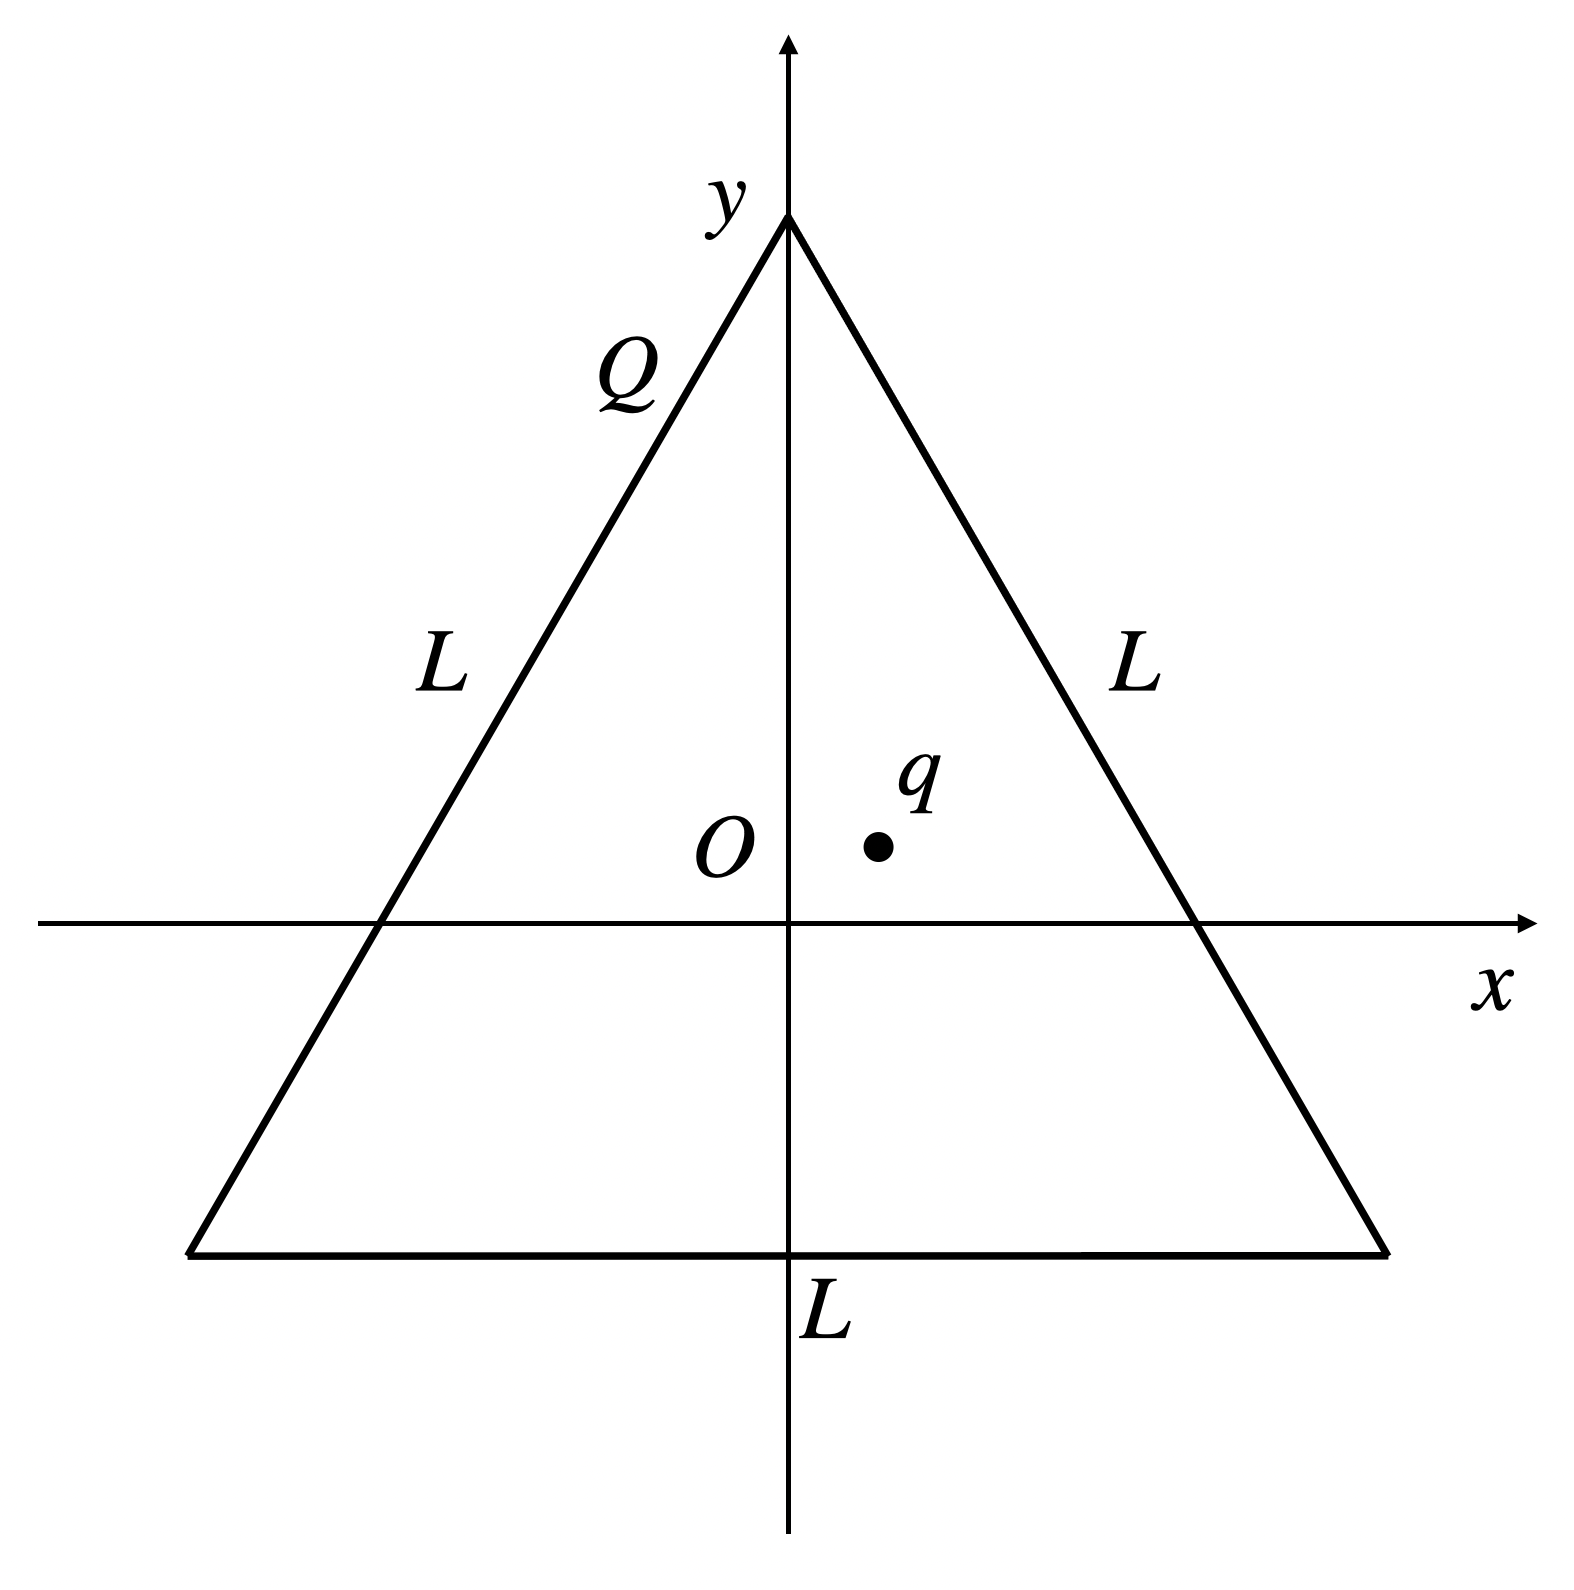
\includegraphics[width=0.5\textwidth]{Fig_P13.png}
\end{center}

\noindent So using the Coulomb law, we can calculate the voltage of the massive point is:	
	
\begin{align*}
	\varphi (x,y)= & \frac{Q}{12 \pi \varepsilon_0 L} \left[ \sinh^{-1} \left( \sqrt{3} \frac{1 + \frac{2x}{L}}{1 + \frac{2\sqrt{3}y}{L}} \right) + \sinh^{-1} \left( \sqrt{3} \frac{1 - \frac{2x}{L}}{1 + \frac{2\sqrt{3}y}{L}} \right) \right] \\
	+ & \frac{Q}{12 \pi \varepsilon_0 L} \left[ \sinh^{-1} \left( \sqrt{3} \frac{1 + \frac{-x + \sqrt{3} y}{L}}{1 + \frac{-3x -\sqrt{3}y}{L}} \right) + \sinh^{-1} \left( \sqrt{3} \frac{1 - \frac{-x + \sqrt{3} y}{L}}{1 + \frac{-3x -\sqrt{3}y}{L}} \right) \right] \\
	+ & \frac{Q}{12 \pi \varepsilon_0 L} \left[ \sinh^{-1} \left( \sqrt{3} \frac{1 + \frac{-x - \sqrt{3}y}{L}}{1 + \frac{3x - \sqrt{3}y}{L}} \right) + \sinh^{-1} \left( \sqrt{3} \frac{1 - \frac{-x - \sqrt{3}y}{L}}{1 + \frac{3x - \sqrt{3}y}{L}} \right) \right] .
\end{align*}	

\noindent The Lagrangian of this massive point is:
$$ L = \frac{1}{2} m \left( \dot{x}^2 + \dot{y}^2 \right) - q \varphi (x,y) .$$
	
\noindent Euler-Lagrange equation:
\begin{align*}
	& \frac{d}{dt} \left( \frac{ \partial L}{\partial \dot{x} } \right) = \frac{\partial L}{\partial x} \Rightarrow m \ddot{x} = - q \frac{\partial \varphi}{\partial x} \approx - \frac{3\sqrt{3}}{2} \frac{qQ}{\pi \varepsilon_0 L^3} x. \\
	& \frac{d}{dt} \left( \frac{ \partial L}{\partial \dot{y} } \right) = \frac{\partial L}{\partial y} \Rightarrow m \ddot{y} = - q \frac{\partial \varphi}{\partial y} \approx - \frac{3\sqrt{3}}{2} \frac{qQ}{\pi \varepsilon_0 L^3} y.
\end{align*}

\noindent Therefore, if $qQ>0$, the massive point will oscillate with frequency $f= \frac{1}{2\pi} \sqrt{ \frac{3\sqrt{3}}{2} \frac{qQ}{\pi \varepsilon_0 m L^3} }$. This oscillation doesn't depend on the direction of displacement on the plane of the triangle.

\noindent With three dimensions, when the massive point have a small displacement, there is a force effect on it along the $z$ axis:
$$F(z) \approx 3 \sqrt{3} \frac{qQ}{\pi \varepsilon_0 L^3} z.$$
\noindent So, we can see that in this case, $z=0$ isn't stable equilibrium.

\noindent Similarly, if $qQ<0$, $z=0$ is a stable equilibrium, but the center of triangle is not. Therefore, we can't make any frame made of insulating wire from which the charge cannot ‘escape’!






\end{document}
